\section{Modelos clásicos de inteligencia artificial y sus limitaciones}
\label{sec:redes_clasicas}

Esta sección presenta las arquitecturas de redes neuronales abordadas en la
cátedra, analizando sus principios de funcionamiento y las limitaciones que
las hacen insuficientes para el procesamiento del lenguaje natural. Al final
se presenta una tabla comparativa que sintetiza el contraste con la arquitectura
Transformer.

%------------------------------------------------------------
\subsection{El perceptrón}
\label{subsec:perceptron}

El perceptrón es la unidad computacional más elemental de las redes
neuronales artificiales~\cite{goodfellow2016deeplearning}. Recibe un vector
de entradas $\bm{x} \in \mathbb{R}^n$, calcula una combinación lineal
ponderada con pesos $\bm{w}$ y un sesgo $b$, y aplica una función de
activación $\varphi$ para producir la salida $y$:

\begin{equation}
    y = \varphi\!\left(\sum_{i=1}^{n} w_i x_i + b\right)
\end{equation}

% ============================================================
% fig_perceptron.tex: Diagrama del perceptrón
% Uso: % ============================================================
% fig_perceptron.tex: Diagrama del perceptrón
% Uso: % ============================================================
% fig_perceptron.tex: Diagrama del perceptrón
% Uso: \input{figures/fig_perceptron}
% ============================================================
\begin{figure}[H]
\centering
\begin{tikzpicture}[
    node distance=1.4cm,
    input/.style={circle, draw=gray!60, fill=gray!15, minimum size=0.8cm, font=\small},
    neuron/.style={circle, draw=blue!60, fill=blue!10, minimum size=1.0cm, font=\small\bfseries},
    output/.style={circle, draw=green!60!black, fill=green!10, minimum size=0.8cm, font=\small},
    arrow/.style={-{Stealth}, thick}
]

% Entradas
\node[input] (x1) at (0, 2)   {$x_1$};
\node[input] (x2) at (0, 0.7) {$x_2$};
\node        (xd) at (0,-0.1) {$\vdots$};
\node[input] (xn) at (0,-1)   {$x_n$};

% Neurona
\node[neuron] (n) at (3, 0.7) {$\Sigma$};

% Salida
\node[output] (y) at (5.5, 0.7) {$y$};

% Bias
\node[input] (b) at (1.5, -1.8) {$b$};

% Función de activación (caja)
\node[draw=orange!70, fill=orange!10, rounded corners, minimum width=1.1cm,
      minimum height=0.7cm, font=\small] (phi) at (4.4, 0.7) {$\varphi$};

% Flechas entradas → neurona
\draw[arrow] (x1) -- node[above, font=\tiny] {$w_1$} (n);
\draw[arrow] (x2) -- node[above, font=\tiny] {$w_2$} (n);
\draw[arrow] (xn) -- node[below, font=\tiny] {$w_n$} (n);
\draw[arrow] (b)  -- (n);

% Neurona → activación → salida
\draw[arrow] (n)   -- (phi);
\draw[arrow] (phi) -- (y);

% Etiquetas
\node[font=\footnotesize, gray] at (0, -2.2) {Entradas};
\node[font=\footnotesize, gray] at (3, -2.2) {Suma ponderada};
\node[font=\footnotesize, gray] at (5.5, -2.2) {Salida};

\end{tikzpicture}
\caption{Estructura del perceptrón. Las entradas $x_i$ se combinan linealmente
con pesos $w_i$ y un sesgo $b$; la suma se pasa por una función de activación
$\varphi$ para producir la salida $y$.}
\label{fig:perceptron}
\end{figure}

% ============================================================
\begin{figure}[H]
\centering
\begin{tikzpicture}[
    node distance=1.4cm,
    input/.style={circle, draw=gray!60, fill=gray!15, minimum size=0.8cm, font=\small},
    neuron/.style={circle, draw=blue!60, fill=blue!10, minimum size=1.0cm, font=\small\bfseries},
    output/.style={circle, draw=green!60!black, fill=green!10, minimum size=0.8cm, font=\small},
    arrow/.style={-{Stealth}, thick}
]

% Entradas
\node[input] (x1) at (0, 2)   {$x_1$};
\node[input] (x2) at (0, 0.7) {$x_2$};
\node        (xd) at (0,-0.1) {$\vdots$};
\node[input] (xn) at (0,-1)   {$x_n$};

% Neurona
\node[neuron] (n) at (3, 0.7) {$\Sigma$};

% Salida
\node[output] (y) at (5.5, 0.7) {$y$};

% Bias
\node[input] (b) at (1.5, -1.8) {$b$};

% Función de activación (caja)
\node[draw=orange!70, fill=orange!10, rounded corners, minimum width=1.1cm,
      minimum height=0.7cm, font=\small] (phi) at (4.4, 0.7) {$\varphi$};

% Flechas entradas → neurona
\draw[arrow] (x1) -- node[above, font=\tiny] {$w_1$} (n);
\draw[arrow] (x2) -- node[above, font=\tiny] {$w_2$} (n);
\draw[arrow] (xn) -- node[below, font=\tiny] {$w_n$} (n);
\draw[arrow] (b)  -- (n);

% Neurona → activación → salida
\draw[arrow] (n)   -- (phi);
\draw[arrow] (phi) -- (y);

% Etiquetas
\node[font=\footnotesize, gray] at (0, -2.2) {Entradas};
\node[font=\footnotesize, gray] at (3, -2.2) {Suma ponderada};
\node[font=\footnotesize, gray] at (5.5, -2.2) {Salida};

\end{tikzpicture}
\caption{Estructura del perceptrón. Las entradas $x_i$ se combinan linealmente
con pesos $w_i$ y un sesgo $b$; la suma se pasa por una función de activación
$\varphi$ para producir la salida $y$.}
\label{fig:perceptron}
\end{figure}

% ============================================================
\begin{figure}[H]
\centering
\begin{tikzpicture}[
    node distance=1.4cm,
    input/.style={circle, draw=gray!60, fill=gray!15, minimum size=0.8cm, font=\small},
    neuron/.style={circle, draw=blue!60, fill=blue!10, minimum size=1.0cm, font=\small\bfseries},
    output/.style={circle, draw=green!60!black, fill=green!10, minimum size=0.8cm, font=\small},
    arrow/.style={-{Stealth}, thick}
]

% Entradas
\node[input] (x1) at (0, 2)   {$x_1$};
\node[input] (x2) at (0, 0.7) {$x_2$};
\node        (xd) at (0,-0.1) {$\vdots$};
\node[input] (xn) at (0,-1)   {$x_n$};

% Neurona
\node[neuron] (n) at (3, 0.7) {$\Sigma$};

% Salida
\node[output] (y) at (5.5, 0.7) {$y$};

% Bias
\node[input] (b) at (1.5, -1.8) {$b$};

% Función de activación (caja)
\node[draw=orange!70, fill=orange!10, rounded corners, minimum width=1.1cm,
      minimum height=0.7cm, font=\small] (phi) at (4.4, 0.7) {$\varphi$};

% Flechas entradas → neurona
\draw[arrow] (x1) -- node[above, font=\tiny] {$w_1$} (n);
\draw[arrow] (x2) -- node[above, font=\tiny] {$w_2$} (n);
\draw[arrow] (xn) -- node[below, font=\tiny] {$w_n$} (n);
\draw[arrow] (b)  -- (n);

% Neurona → activación → salida
\draw[arrow] (n)   -- (phi);
\draw[arrow] (phi) -- (y);

% Etiquetas
\node[font=\footnotesize, gray] at (0, -2.2) {Entradas};
\node[font=\footnotesize, gray] at (3, -2.2) {Suma ponderada};
\node[font=\footnotesize, gray] at (5.5, -2.2) {Salida};

\end{tikzpicture}
\caption{Estructura del perceptrón. Las entradas $x_i$ se combinan linealmente
con pesos $w_i$ y un sesgo $b$; la suma se pasa por una función de activación
$\varphi$ para producir la salida $y$.}
\label{fig:perceptron}
\end{figure}


El conocimiento del perceptrón reside íntegramente en los pesos $\bm{w}$,
que se ajustan durante el entrenamiento. Sin embargo, su capacidad
representacional es fundamentalmente limitada: solo puede producir
fronteras de decisión lineales en el espacio de entrada. Cualquier problema
con estructura no lineal —como la función XOR— no puede ser resuelto por
un único perceptrón. Esta limitación motivó el desarrollo del perceptrón
multicapa.

%------------------------------------------------------------
\subsection{El perceptrón multicapa, backpropagation y descenso del gradiente}
\label{subsec:mlp}

El perceptrón multicapa (MLP) supera las limitaciones del perceptrón simple
apilando capas de neuronas con funciones de activación no lineales. El teorema
de aproximación universal establece que un MLP con al menos una capa oculta
suficientemente amplia puede aproximar cualquier función continua en un
compacto~\cite{goodfellow2016deeplearning}.

\begin{figure}[H]
\centering
\begin{tikzpicture}[
    neuron/.style={circle, draw=blue!50, fill=blue!8, minimum size=0.75cm, font=\scriptsize},
    out/.style={circle, draw=green!60!black, fill=green!8, minimum size=0.75cm, font=\scriptsize},
    arrow/.style={-{Stealth}, thick},
    back/.style={-{Stealth}, thick, dashed, red!70},
    layer/.style={font=\small\bfseries, gray}
]

% Capa de entrada (3 nodos)
\foreach \i/\y in {1/2, 2/0.7, 3/-0.7}{
    \node[neuron] (i\i) at (0, \y) {$x_{\i}$};
}

% Capa oculta 1 (4 nodos)
\foreach \i/\y in {1/2.7, 2/1.2, 3/-0.2, 4/-1.5}{
    \node[neuron] (h1\i) at (2.5, \y) {};
}

% Capa oculta 2 (4 nodos)
\foreach \i/\y in {1/2.7, 2/1.2, 3/-0.2, 4/-1.5}{
    \node[neuron] (h2\i) at (5, \y) {};
}

% Capa de salida (2 nodos)
\foreach \i/\y in {1/1.0, 2/-0.3}{
    \node[out=45, in=135] (o\i) at (7.5, \y) {$y_{\i}$};
}

% Conexiones entrada → oculta1
\foreach \i in {1,2,3}{
    \foreach \j in {1,2,3,4}{
        \draw[-{Stealth}, gray!50, thin] (i\i) -- (h1\j);
    }
}
% Conexiones oculta1 → oculta2
\foreach \i in {1,2,3,4}{
    \foreach \j in {1,2,3,4}{
        \draw[-{Stealth}, gray!50, thin] (h1\i) -- (h2\j);
    }
}
% Conexiones oculta2 → salida
\foreach \i in {1,2,3,4}{
    \foreach \j in {1,2}{
        \draw[-{Stealth}, gray!50, thin] (h2\i) -- (o\j);
    }
}

% Flecha de forward pass (arriba)
\draw[arrow, blue!70] (-0.6, 3.5) -- node[above, font=\small] {Forward pass $\longrightarrow$} (8.1, 3.5);

% Flecha de backward pass (abajo)
\draw[back] (8.1, -2.3) -- node[below, font=\small] {$\longleftarrow$ Backpropagation $\nabla\mathcal{L}$} (-0.6, -2.3);

% Etiquetas de capas
\node[layer] at (0,   -3.3) {Entrada};
\node[layer] at (2.5, -3.3) {Oculta 1};
\node[layer] at (5,   -3.3) {Oculta 2};
\node[layer] at (7.5, -3.3) {Salida};

\end{tikzpicture}
\caption{Perceptrón multicapa (MLP). El \textit{forward pass} propaga la
información de izquierda a derecha. La retropropagación (\textit{backpropagation})
calcula los gradientes de la pérdida $\mathcal{L}$ en sentido inverso,
actualizando los pesos mediante descenso del gradiente.}
\label{fig:mlp}
\end{figure}


\subsubsection*{Backpropagation}

El entrenamiento del MLP se realiza mediante el algoritmo de retropropagación
del error (\textit{backpropagation}), que calcula eficientemente el gradiente
de la función de pérdida $\mathcal{L}$ respecto a cada parámetro de la red
aplicando la regla de la cadena en sentido inverso a través de las capas:

\begin{equation}
    \frac{\partial \mathcal{L}}{\partial w_{ij}^{(l)}} =
    \frac{\partial \mathcal{L}}{\partial a_j^{(l)}} \cdot
    \frac{\partial a_j^{(l)}}{\partial w_{ij}^{(l)}}
\end{equation}

\noindent donde $a_j^{(l)}$ es la activación de la neurona $j$ en la capa $l$
y $w_{ij}^{(l)}$ es el peso que la conecta con la neurona $i$ de la capa
anterior. El proceso recorre la red de salida hacia entrada (\textit{backward}),
acumulando gradientes en cada capa.

\subsubsection*{Descenso del gradiente}

Los gradientes obtenidos por backpropagation se usan para actualizar los
parámetros mediante descenso del gradiente. La regla de actualización es:

\begin{equation}
    w \leftarrow w - \eta \, \frac{\partial \mathcal{L}}{\partial w}
\end{equation}

\noindent donde $\eta > 0$ es la \textit{tasa de aprendizaje}. Intuitivamente,
cada actualización mueve los parámetros en la dirección que reduce la pérdida.
Si $\eta$ es demasiado grande el proceso puede divergir u oscilar; si es
demasiado pequeño, la convergencia es lenta o puede quedar atrapada en
mínimos locales subóptimos.

% ============================================================
% fig_gradient_descent.tex: Descenso del gradiente
% Uso: % ============================================================
% fig_gradient_descent.tex: Descenso del gradiente
% Uso: % ============================================================
% fig_gradient_descent.tex: Descenso del gradiente
% Uso: \input{figures/fig_gradient_descent}
% ============================================================
\begin{figure}[H]
\centering
\begin{tikzpicture}[scale=1.1]

% Ejes
\draw[-{Stealth}, thick] (-0.3, 0) -- (6.5, 0) node[right] {$w$};
\draw[-{Stealth}, thick] (0, -0.3) -- (0, 4.2) node[above] {$\mathcal{L}(w)$};

% Curva de pérdida (parábola suavizada)
\draw[blue!70, very thick, domain=0.3:6.1, samples=80]
    plot (\x, {0.35*(\x-3.2)^2 + 0.5});

% Mínimo
\fill[green!60!black] (3.2, 0.5) circle (3pt) node[below right, font=\small] {mínimo};

% Puntos del descenso
\coordinate (p1) at (1.0, 2.34);
\coordinate (p2) at (1.7, 1.44);
\coordinate (p3) at (2.3, 0.87);
\coordinate (p4) at (2.75, 0.59);
\coordinate (p5) at (3.05, 0.51);

\fill[red!70]    (p1) circle (3pt);
\fill[red!60]    (p2) circle (3pt);
\fill[orange!80] (p3) circle (3pt);
\fill[orange!60] (p4) circle (3pt);
\fill[yellow!80!orange] (p5) circle (3pt);

% Flechas de actualización
\draw[-{Stealth}, red!60, thick]    (p1) -- (p2);
\draw[-{Stealth}, red!40, thick]    (p2) -- (p3);
\draw[-{Stealth}, orange!80, thick] (p3) -- (p4);
\draw[-{Stealth}, orange!50, thick] (p4) -- (p5);

% Etiqueta tasa de aprendizaje
\draw[dashed, gray] (1.0, 0) -- (p1);
\draw[dashed, gray] (1.7, 0) -- (p2);
\node[font=\tiny, gray] at (1.35, -0.2) {$\eta \cdot \nabla\mathcal{L}$};
\draw[{Stealth}-{Stealth}, gray, thin] (1.05, -0.15) -- (1.65, -0.15);

% Fórmula
\node[draw=blue!30, fill=blue!5, rounded corners, font=\small,
      inner sep=6pt] at (5.0, 3.5)
      {$w \leftarrow w - \eta \dfrac{\partial \mathcal{L}}{\partial w}$};

\node[font=\footnotesize, gray] at (3.2, -0.5) {$w^*$};

\end{tikzpicture}
\caption{Descenso del gradiente. Partiendo de un valor inicial de $w$, cada
iteración actualiza el parámetro en dirección opuesta al gradiente de la
pérdida $\mathcal{L}$, con magnitud controlada por la tasa de aprendizaje
$\eta$. El proceso converge progresivamente al mínimo $w^*$.}
\label{fig:gradient_descent}
\end{figure}

% ============================================================
\begin{figure}[H]
\centering
\begin{tikzpicture}[scale=1.1]

% Ejes
\draw[-{Stealth}, thick] (-0.3, 0) -- (6.5, 0) node[right] {$w$};
\draw[-{Stealth}, thick] (0, -0.3) -- (0, 4.2) node[above] {$\mathcal{L}(w)$};

% Curva de pérdida (parábola suavizada)
\draw[blue!70, very thick, domain=0.3:6.1, samples=80]
    plot (\x, {0.35*(\x-3.2)^2 + 0.5});

% Mínimo
\fill[green!60!black] (3.2, 0.5) circle (3pt) node[below right, font=\small] {mínimo};

% Puntos del descenso
\coordinate (p1) at (1.0, 2.34);
\coordinate (p2) at (1.7, 1.44);
\coordinate (p3) at (2.3, 0.87);
\coordinate (p4) at (2.75, 0.59);
\coordinate (p5) at (3.05, 0.51);

\fill[red!70]    (p1) circle (3pt);
\fill[red!60]    (p2) circle (3pt);
\fill[orange!80] (p3) circle (3pt);
\fill[orange!60] (p4) circle (3pt);
\fill[yellow!80!orange] (p5) circle (3pt);

% Flechas de actualización
\draw[-{Stealth}, red!60, thick]    (p1) -- (p2);
\draw[-{Stealth}, red!40, thick]    (p2) -- (p3);
\draw[-{Stealth}, orange!80, thick] (p3) -- (p4);
\draw[-{Stealth}, orange!50, thick] (p4) -- (p5);

% Etiqueta tasa de aprendizaje
\draw[dashed, gray] (1.0, 0) -- (p1);
\draw[dashed, gray] (1.7, 0) -- (p2);
\node[font=\tiny, gray] at (1.35, -0.2) {$\eta \cdot \nabla\mathcal{L}$};
\draw[{Stealth}-{Stealth}, gray, thin] (1.05, -0.15) -- (1.65, -0.15);

% Fórmula
\node[draw=blue!30, fill=blue!5, rounded corners, font=\small,
      inner sep=6pt] at (5.0, 3.5)
      {$w \leftarrow w - \eta \dfrac{\partial \mathcal{L}}{\partial w}$};

\node[font=\footnotesize, gray] at (3.2, -0.5) {$w^*$};

\end{tikzpicture}
\caption{Descenso del gradiente. Partiendo de un valor inicial de $w$, cada
iteración actualiza el parámetro en dirección opuesta al gradiente de la
pérdida $\mathcal{L}$, con magnitud controlada por la tasa de aprendizaje
$\eta$. El proceso converge progresivamente al mínimo $w^*$.}
\label{fig:gradient_descent}
\end{figure}

% ============================================================
\begin{figure}[H]
\centering
\begin{tikzpicture}[scale=1.1]

% Ejes
\draw[-{Stealth}, thick] (-0.3, 0) -- (6.5, 0) node[right] {$w$};
\draw[-{Stealth}, thick] (0, -0.3) -- (0, 4.2) node[above] {$\mathcal{L}(w)$};

% Curva de pérdida (parábola suavizada)
\draw[blue!70, very thick, domain=0.3:6.1, samples=80]
    plot (\x, {0.35*(\x-3.2)^2 + 0.5});

% Mínimo
\fill[green!60!black] (3.2, 0.5) circle (3pt) node[below right, font=\small] {mínimo};

% Puntos del descenso
\coordinate (p1) at (1.0, 2.34);
\coordinate (p2) at (1.7, 1.44);
\coordinate (p3) at (2.3, 0.87);
\coordinate (p4) at (2.75, 0.59);
\coordinate (p5) at (3.05, 0.51);

\fill[red!70]    (p1) circle (3pt);
\fill[red!60]    (p2) circle (3pt);
\fill[orange!80] (p3) circle (3pt);
\fill[orange!60] (p4) circle (3pt);
\fill[yellow!80!orange] (p5) circle (3pt);

% Flechas de actualización
\draw[-{Stealth}, red!60, thick]    (p1) -- (p2);
\draw[-{Stealth}, red!40, thick]    (p2) -- (p3);
\draw[-{Stealth}, orange!80, thick] (p3) -- (p4);
\draw[-{Stealth}, orange!50, thick] (p4) -- (p5);

% Etiqueta tasa de aprendizaje
\draw[dashed, gray] (1.0, 0) -- (p1);
\draw[dashed, gray] (1.7, 0) -- (p2);
\node[font=\tiny, gray] at (1.35, -0.2) {$\eta \cdot \nabla\mathcal{L}$};
\draw[{Stealth}-{Stealth}, gray, thin] (1.05, -0.15) -- (1.65, -0.15);

% Fórmula
\node[draw=blue!30, fill=blue!5, rounded corners, font=\small,
      inner sep=6pt] at (5.0, 3.5)
      {$w \leftarrow w - \eta \dfrac{\partial \mathcal{L}}{\partial w}$};

\node[font=\footnotesize, gray] at (3.2, -0.5) {$w^*$};

\end{tikzpicture}
\caption{Descenso del gradiente. Partiendo de un valor inicial de $w$, cada
iteración actualiza el parámetro en dirección opuesta al gradiente de la
pérdida $\mathcal{L}$, con magnitud controlada por la tasa de aprendizaje
$\eta$. El proceso converge progresivamente al mínimo $w^*$.}
\label{fig:gradient_descent}
\end{figure}


\subsubsection*{Limitaciones para el modelado de secuencias}

A pesar de su capacidad expresiva, los MLPs presentan limitaciones
estructurales que los hacen inadecuados para procesar lenguaje natural:

\begin{itemize}
    \item \textbf{Entradas de tamaño fijo.} El MLP requiere que la dimensión
    de la entrada esté fija en el momento del diseño. Para modelar texto,
    esto implica definir una ventana de contexto de longitud constante,
    truncando o rellenando todas las secuencias a esa longitud. Esto hace
    imposible adaptarse a oraciones de longitud variable sin pérdida de
    información~\cite{bengio2003neural}.

    \item \textbf{Ausencia de codificación del orden.} La posición de cada
    elemento en el vector de entrada no tiene representación interna
    diferenciada: si se permutan los elementos, la red no puede distinguir
    el nuevo orden del original. Para el lenguaje esto es crítico: \textit{``el
    perro muerde al hombre''} y \textit{``el hombre muerde al perro''} son
    semánticamente opuestas, pero un MLP que reciba las mismas palabras en
    distinto orden producirá la misma activación interna si no hay codificación
    posicional explícita~\cite{goodfellow2016deeplearning}.

    \item \textbf{Sin mecanismo relacional dinámico.} En un MLP los pesos son
    estáticos: la red no puede decidir en tiempo de inferencia a qué parte de
    la entrada prestarle más atención según el contexto. Dos palabras pueden
    ser muy relevantes entre sí en una oración y completamente irrelevantes
    en otra, pero el modelo las procesa siempre con los mismos pesos.

    \item \textbf{Dependencias limitadas al tamaño de la ventana.} Toda
    relación que exija considerar elementos separados por más posiciones que
    el ancho de la ventana es inaccesible para el modelo. En textos largos,
    esto descarta dependencias fundamentales: el sujeto de una oración puede
    estar decenas de palabras antes del verbo que lo acompaña~\cite{bengio2003neural}.
\end{itemize}

%------------------------------------------------------------
\subsection{Redes de Hopfield}
\label{subsec:hopfield}

Las redes de Hopfield~\cite{hopfield1982neural} son redes recurrentes
completamente conectadas diseñadas como modelos de \textit{memoria asociativa}:
dado un patrón de entrada incompleto o ruidoso, la red recupera el patrón
almacenado más cercano. Cada unidad $s_i \in \{-1, +1\}$ se conecta
simétricamente con todas las demás ($w_{ij} = w_{ji}$), y la dinámica del
sistema minimiza una función de energía global:

\begin{equation}
    E = -\frac{1}{2} \sum_{i \neq j} w_{ij} \, s_i \, s_j
\end{equation}

La regla de actualización de cada neurona es:

\begin{equation}
    s_i \leftarrow \text{sgn}\!\left(\sum_{j} w_{ij} \, s_j\right)
\end{equation}

La red converge cuando ninguna actualización reduce la energía, es decir,
cuando alcanza un mínimo local. Estos mínimos corresponden a los patrones
almacenados durante el entrenamiento. La Figura~\ref{fig:hopfield_energia}
muestra este paisaje de energía conceptualmente.

% ============================================================
% fig_hopfield_energia.tex — Paisaje de energía de Hopfield
% ============================================================
\begin{figure}[H]
\centering
\begin{tikzpicture}[scale=1.1]

% Ejes
\draw[-{Stealth}, thick] (-0.3, 0) -- (7.2, 0) node[right, font=\small] {espacio de estados};
\draw[-{Stealth}, thick] (0, -0.3) -- (0, 4.0) node[above, font=\small] {$E$};

% Curva de energía con varios mínimos locales
% Fix: usar grados directamente (sin sufijo r) con factores escalados
\draw[blue!70, very thick, domain=0.2:7.0, samples=200]
    plot (\x, {
        0.6*sin(51.43*\x) +
        0.4*sin(102.86*\x) +
        0.3*cos(77.14*\x) +
        1.8
    });

% Mínimos (patrones almacenados)
\fill[green!60!black] (1.05, 0.82) circle (3.5pt);
\fill[green!60!black] (3.55, 0.62) circle (3.5pt);
\fill[green!60!black] (5.90, 0.95) circle (3.5pt);

\node[green!50!black, font=\footnotesize, above right] at (1.05, 0.82) {patrón $\xi^1$};
\node[green!50!black, font=\footnotesize, above right] at (3.55, 0.62) {patrón $\xi^2$};
\node[green!50!black, font=\footnotesize, above right] at (5.90, 0.95) {patrón $\xi^3$};

% Estado inicial ruidoso → convergencia hacia mínimo
\fill[red!70]    (2.3, 2.85) circle (3pt) node[above, font=\footnotesize, red!70] {entrada ruidosa};
\draw[-{Stealth}, red!60, thick, dashed]
    (2.3, 2.85) .. controls (2.1, 2.0) and (1.7, 1.4) .. (1.05, 0.85);
\node[red!60, font=\tiny] at (1.5, 1.9) {convergencia};

% Etiqueta eje Y
\node[font=\footnotesize, gray, rotate=90] at (-0.55, 2.0) {Energía $E$};

\end{tikzpicture}
\caption{Paisaje de energía de una red de Hopfield. Cada mínimo local corresponde
a un patrón almacenado $\xi^k$. Ante una entrada ruidosa o incompleta, la dinámica
de la red desciende por el gradiente de energía hasta converger al mínimo más
cercano, recuperando el patrón original.}
\label{fig:hopfield_energia}
\end{figure}


\subsubsection*{Ejemplo numérico: recuperación de un patrón}

Para ilustrar el mecanismo, considérese una red de 4 neuronas con un patrón
almacenado $\xi^1 = [+1,-1,+1,-1]$. Los pesos se calculan mediante la regla
de Hebb:
$w_{ij} = \frac{1}{n} \sum_\mu \xi_i^\mu \xi_j^\mu$.
Si se presenta la entrada ruidosa $\bm{s} = [+1,+1,+1,-1]$ (bit $s_2$
invertido), la regla de actualización corrige el error en una sola iteración,
recuperando el patrón original.

% ============================================================
% fig_hopfield_ejemplo.tex: Ejemplo numérico paso a paso (4 neuronas)
% ============================================================
\begin{figure}[H]
\centering
\begin{tikzpicture}[
    cell/.style={draw, minimum width=0.55cm, minimum height=0.55cm, font=\footnotesize},
    on/.style={cell, fill=blue!60, text=white},
    off/.style={cell, fill=gray!20},
    lbl/.style={font=\footnotesize\bfseries},
    stepnum/.style={font=\small\bfseries, text=blue!70},
    arrow/.style={-{Stealth}, thick, gray}
]

% ── Fila 0: encabezados ─────────────────────────────────────
\node[lbl] at (-1.8, 3.8) {Paso};
\node[lbl] at ( 0.4, 3.8) {Estado $\bm{s}$};
\node[lbl] at ( 3.6, 3.8) {Descripción};

% ── Paso 0: patrón almacenado ───────────────────────────────
\node[stepnum]  at (-1.8, 3.0) {0};
\foreach \v/\i in {+1/0, -1/1, +1/2, -1/3}{
    \pgfmathparse{(\v>0)?1:0}
    \ifnum\pgfmathresult=1
        \node[on]  at (\i*0.65, 3.0) {\v};
    \else
        \node[off] at (\i*0.65, 3.0) {\v};
    \fi
}
\node[font=\footnotesize, align=left] at (5.9, 3.0)
    {Patrón almacenado $\xi^1 = [+1,-1,+1,-1]$};

% ── Separador ───────────────────────────────────────────────
\draw[dashed, gray!50] (-2.5, 2.55) -- (5.0, 2.55);

% ── Paso 1: entrada ruidosa ─────────────────────────────────
\node[stepnum]  at (-1.8, 2.1) {1};
\foreach \v/\i in {+1/0, +1/1, +1/2, -1/3}{
    \pgfmathparse{(\v>0)?1:0}
    \ifnum\pgfmathresult=1
        \node[on]  at (\i*0.65, 2.1) {\v};
    \else
        \node[off] at (\i*0.65, 2.1) {\v};
    \fi
}
\draw[red!70, very thick] (0.65-0.27, 2.1-0.27) rectangle (0.65+0.27, 2.1+0.27);
\node[font=\footnotesize, align=left] at (5.6, 2.1)
    {Entrada ruidosa: $s_2$ invertido {\color{red!70}$\leftarrow$ error}};

% ── Flecha de actualización ─────────────────────────────────
\draw[arrow] (0.95, 1.78) -- (0.95, 1.35);
\node[font=\tiny, gray] at (2.5, 1.57) {actualización: $s_i \leftarrow \text{sgn}\!\left(\sum_j w_{ij} s_j\right)$};

% ── Paso 2: después de una iteración ────────────────────────
\node[stepnum]  at (-1.8, 1.05) {2};
\foreach \v/\i in {+1/0, -1/1, +1/2, -1/3}{
    \pgfmathparse{(\v>0)?1:0}
    \ifnum\pgfmathresult=1
        \node[on]  at (\i*0.65, 1.05) {\v};
    \else
        \node[off] at (\i*0.65, 1.05) {\v};
    \fi
}
\node[font=\footnotesize, align=left] at (6.0, 1.05)
    {Tras actualizar $s_2$: patrón recuperado $\xi^1$ {\color{green!60!black}$\checkmark$}};

% ── Estado estable ───────────────────────────────────────────
\draw[dashed, gray!50] (-2.5, 0.6) -- (6.8, 0.6);
\node[font=\footnotesize, gray, align=left] at (2.0, 0.25)
    {Estado estable: $E$ alcanzó mínimo local $\Rightarrow$ la red converge.};

% ── Leyenda ─────────────────────────────────────────────────
\node[on,  label=right:{\footnotesize $s_i = +1$ (activa)}]  at (-1.2, -0.35) {};
\node[off, label=right:{\footnotesize $s_i = -1$ (inactiva)}] at ( 2.8, -0.35) {};

\end{tikzpicture}
\caption{Ejemplo de recuperación de un patrón en una red de Hopfield con
4 neuronas. El patrón almacenado $\xi^1 = [+1,-1,+1,-1]$ se recupera
correctamente a partir de una versión ruidosa en la que el bit $s_2$ estaba
invertido. La regla de actualización $s_i \leftarrow \text{sgn}\!\left(\sum_j w_{ij} s_j\right)$
corrige el error en una sola iteración.}
\label{fig:hopfield_ejemplo}
\end{figure}


\subsubsection*{Conexión con los Transformers}

La red de Hopfield introduce un concepto que reaparecerá de forma central en
los Transformers: la \textit{influencia global entre unidades}. El estado de
cada neurona está determinado por el estado de todas las demás, lo que
constituye una forma primitiva de atención distribuida. Sin embargo, la
capacidad de almacenamiento clásica es limitada (aproximadamente $0.14n$
patrones) y el modelo no está diseñado para representar relaciones
secuenciales. Trabajos recientes han demostrado que el mecanismo de atención
puede interpretarse como una generalización de Hopfield con capacidad de
almacenamiento exponencial~\cite{ramsauer2020hopfield}.

%------------------------------------------------------------
\subsection{Mapas autoorganizados (SOM)}
\label{subsec:som}

Los mapas autoorganizados (SOM), propuestos por Kohonen~\cite{kohonen1990som},
son redes no supervisadas que aprenden a proyectar datos de alta dimensión en
una grilla discreta de baja dimensión (usualmente 2D), preservando la topología
del espacio original. Cada neurona de la grilla tiene asociado un vector de
pesos $\bm{w}_i \in \mathbb{R}^d$ del mismo tamaño que los datos de entrada.

\subsubsection*{Proceso de entrenamiento}

En cada iteración se presenta una muestra $\bm{x}$ y se identifican:

\begin{enumerate}
    \item \textbf{Neurona ganadora (BMU):} aquella cuyo vector de pesos es más
    cercano a $\bm{x}$ en distancia euclidiana:
    $c = \arg\min_i \|\bm{x} - \bm{w}_i\|$.

    \item \textbf{Actualización de la BMU y sus vecinas:} los pesos de la BMU
    y las neuronas en su entorno se acercan a $\bm{x}$:
    \begin{equation}
        \bm{w}_i(t{+}1) = \bm{w}_i(t) + \alpha(t)\,h_{ci}(t)\,
        [\bm{x}(t) - \bm{w}_i(t)]
    \end{equation}
    donde $\alpha(t)$ es la tasa de aprendizaje y $h_{ci}(t)$ es la función
    de vecindad (usualmente gaussiana), que decrece con la distancia en la
    grilla entre la BMU $c$ y la neurona $i$.
\end{enumerate}

Tras muchas iteraciones, neuronas contiguas en la grilla responden a entradas
similares: la topología del espacio de entrada queda reflejada en la grilla 2D.

% ============================================================
% fig_som_proceso.tex: Proceso de entrenamiento SOM (pasos)
% Uso: % ============================================================
% fig_som_proceso.tex: Proceso de entrenamiento SOM (pasos)
% Uso: % ============================================================
% fig_som_proceso.tex: Proceso de entrenamiento SOM (pasos)
% Uso: \input{figures/fig_som_proceso}
% ============================================================
\begin{figure}[H]
\centering
\begin{tikzpicture}[
    neuron/.style={circle, draw=blue!50, fill=blue!8, minimum size=0.55cm},
    bmu/.style={circle, draw=red!70, fill=red!20, minimum size=0.55cm, very thick},
    neighbor/.style={circle, draw=orange!70, fill=orange!10, minimum size=0.55cm, thick},
    input/.style={circle, draw=green!60!black, fill=green!15, minimum size=0.6cm, font=\tiny},
    arrow/.style={-{Stealth}, thick},
    label/.style={font=\small\bfseries, gray}
]

% ─── Grilla 3×3 en t=0 (aleatoria) ──────────────────────────
\node[label] at (1.0, 4.1) {$t = 0$ (inicial)};
\foreach \row in {0,1,2}{
    \foreach \col in {0,1,2}{
        \node[neuron] at (\col*0.9, 3.2-\row*0.9) {};
    }
}
\node[font=\tiny, gray] at (1.0, 0.8) {pesos aleatorios};

% ─── Flecha paso 1 ──────────────────────────────────────────
\draw[arrow, blue!60] (2.4, 2.2) -- (3.2, 2.2);
\node[font=\tiny, align=center, blue!70] at (2.8, 2.55)
    {1. presentar\\entrada $\bm{x}$};

% ─── Grilla con BMU marcada ──────────────────────────────────
\node[label] at (5.0, 4.1) {BMU encontrada};
% Entrada
\node[input] at (5.0, 4.55) {$\bm{x}$};
\foreach \row in {0,1,2}{
    \foreach \col in {0,1,2}{
        \pgfmathparse{int(\row==1 && \col==1)}
        \ifnum\pgfmathresult=1
            \node[bmu]      at (3.6+\col*0.9, 3.2-\row*0.9) {};
        \else
            \pgfmathparse{int(abs(\row-1)<=1 && abs(\col-1)<=1)}
            \ifnum\pgfmathresult=1
                \node[neighbor] at (3.6+\col*0.9, 3.2-\row*0.9) {};
            \else
                \node[neuron]   at (3.6+\col*0.9, 3.2-\row*0.9) {};
            \fi
        \fi
    }
}
\draw[red!60, dashed] (5.0, 4.4) -- (4.5, 2.3);
\node[font=\tiny, gray] at (5.0, 0.8) {BMU=rojo, vecinos=naranja};

% ─── Flecha paso 2 ──────────────────────────────────────────
\draw[arrow, blue!60] (6.4, 2.2) -- (7.2, 2.2);
\node[font=\tiny, align=center, blue!70] at (6.8, 2.55)
    {2. actualizar\\BMU+vecinos};

% ─── Grilla actualizada ─────────────────────────────────────
\node[label] at (9.0, 4.1) {pesos actualizados};
\foreach \row in {0,1,2}{
    \foreach \col in {0,1,2}{
        \pgfmathparse{int(\row==1 && \col==1)}
        \ifnum\pgfmathresult=1
            \node[bmu]      at (7.6+\col*0.9, 3.2-\row*0.9) {};
        \else
            \pgfmathparse{int(abs(\row-1)<=1 && abs(\col-1)<=1)}
            \ifnum\pgfmathresult=1
                \node[neighbor] at (7.6+\col*0.9, 3.2-\row*0.9) {};
            \else
                \node[neuron]   at (7.6+\col*0.9, 3.2-\row*0.9) {};
            \fi
        \fi
    }
}
\node[font=\tiny, gray, align=center] at (9.0, 0.8) {BMU y vecinos se\\acercan a $\bm{x}$};

% ─── Leyenda regla de actualización ─────────────────────────
\node[draw=blue!20, fill=blue!5, rounded corners, font=\footnotesize,
      inner sep=5pt, align=left] at (5.5, -0.5)
      {$\bm{w}_i(t{+}1) = \bm{w}_i(t) + \alpha(t)\, h_{ci}(t)\,[\bm{x}(t) - \bm{w}_i(t)]$};

\end{tikzpicture}
\caption{Proceso de entrenamiento de un SOM en una iteración. (1) Se presenta
una entrada $\bm{x}$ y se identifica la neurona ganadora o \textit{Best Matching
Unit} (BMU, en rojo), la de menor distancia a $\bm{x}$. (2) La BMU y sus
vecinas (naranja) actualizan sus pesos acercándose a $\bm{x}$ según la regla
mostrada, donde $\alpha(t)$ es la tasa de aprendizaje y $h_{ci}(t)$ es la
función de vecindad.}
\label{fig:som_proceso}
\end{figure}

% ============================================================
\begin{figure}[H]
\centering
\begin{tikzpicture}[
    neuron/.style={circle, draw=blue!50, fill=blue!8, minimum size=0.55cm},
    bmu/.style={circle, draw=red!70, fill=red!20, minimum size=0.55cm, very thick},
    neighbor/.style={circle, draw=orange!70, fill=orange!10, minimum size=0.55cm, thick},
    input/.style={circle, draw=green!60!black, fill=green!15, minimum size=0.6cm, font=\tiny},
    arrow/.style={-{Stealth}, thick},
    label/.style={font=\small\bfseries, gray}
]

% ─── Grilla 3×3 en t=0 (aleatoria) ──────────────────────────
\node[label] at (1.0, 4.1) {$t = 0$ (inicial)};
\foreach \row in {0,1,2}{
    \foreach \col in {0,1,2}{
        \node[neuron] at (\col*0.9, 3.2-\row*0.9) {};
    }
}
\node[font=\tiny, gray] at (1.0, 0.8) {pesos aleatorios};

% ─── Flecha paso 1 ──────────────────────────────────────────
\draw[arrow, blue!60] (2.4, 2.2) -- (3.2, 2.2);
\node[font=\tiny, align=center, blue!70] at (2.8, 2.55)
    {1. presentar\\entrada $\bm{x}$};

% ─── Grilla con BMU marcada ──────────────────────────────────
\node[label] at (5.0, 4.1) {BMU encontrada};
% Entrada
\node[input] at (5.0, 4.55) {$\bm{x}$};
\foreach \row in {0,1,2}{
    \foreach \col in {0,1,2}{
        \pgfmathparse{int(\row==1 && \col==1)}
        \ifnum\pgfmathresult=1
            \node[bmu]      at (3.6+\col*0.9, 3.2-\row*0.9) {};
        \else
            \pgfmathparse{int(abs(\row-1)<=1 && abs(\col-1)<=1)}
            \ifnum\pgfmathresult=1
                \node[neighbor] at (3.6+\col*0.9, 3.2-\row*0.9) {};
            \else
                \node[neuron]   at (3.6+\col*0.9, 3.2-\row*0.9) {};
            \fi
        \fi
    }
}
\draw[red!60, dashed] (5.0, 4.4) -- (4.5, 2.3);
\node[font=\tiny, gray] at (5.0, 0.8) {BMU=rojo, vecinos=naranja};

% ─── Flecha paso 2 ──────────────────────────────────────────
\draw[arrow, blue!60] (6.4, 2.2) -- (7.2, 2.2);
\node[font=\tiny, align=center, blue!70] at (6.8, 2.55)
    {2. actualizar\\BMU+vecinos};

% ─── Grilla actualizada ─────────────────────────────────────
\node[label] at (9.0, 4.1) {pesos actualizados};
\foreach \row in {0,1,2}{
    \foreach \col in {0,1,2}{
        \pgfmathparse{int(\row==1 && \col==1)}
        \ifnum\pgfmathresult=1
            \node[bmu]      at (7.6+\col*0.9, 3.2-\row*0.9) {};
        \else
            \pgfmathparse{int(abs(\row-1)<=1 && abs(\col-1)<=1)}
            \ifnum\pgfmathresult=1
                \node[neighbor] at (7.6+\col*0.9, 3.2-\row*0.9) {};
            \else
                \node[neuron]   at (7.6+\col*0.9, 3.2-\row*0.9) {};
            \fi
        \fi
    }
}
\node[font=\tiny, gray, align=center] at (9.0, 0.8) {BMU y vecinos se\\acercan a $\bm{x}$};

% ─── Leyenda regla de actualización ─────────────────────────
\node[draw=blue!20, fill=blue!5, rounded corners, font=\footnotesize,
      inner sep=5pt, align=left] at (5.5, -0.5)
      {$\bm{w}_i(t{+}1) = \bm{w}_i(t) + \alpha(t)\, h_{ci}(t)\,[\bm{x}(t) - \bm{w}_i(t)]$};

\end{tikzpicture}
\caption{Proceso de entrenamiento de un SOM en una iteración. (1) Se presenta
una entrada $\bm{x}$ y se identifica la neurona ganadora o \textit{Best Matching
Unit} (BMU, en rojo), la de menor distancia a $\bm{x}$. (2) La BMU y sus
vecinas (naranja) actualizan sus pesos acercándose a $\bm{x}$ según la regla
mostrada, donde $\alpha(t)$ es la tasa de aprendizaje y $h_{ci}(t)$ es la
función de vecindad.}
\label{fig:som_proceso}
\end{figure}

% ============================================================
\begin{figure}[H]
\centering
\begin{tikzpicture}[
    neuron/.style={circle, draw=blue!50, fill=blue!8, minimum size=0.55cm},
    bmu/.style={circle, draw=red!70, fill=red!20, minimum size=0.55cm, very thick},
    neighbor/.style={circle, draw=orange!70, fill=orange!10, minimum size=0.55cm, thick},
    input/.style={circle, draw=green!60!black, fill=green!15, minimum size=0.6cm, font=\tiny},
    arrow/.style={-{Stealth}, thick},
    label/.style={font=\small\bfseries, gray}
]

% ─── Grilla 3×3 en t=0 (aleatoria) ──────────────────────────
\node[label] at (1.0, 4.1) {$t = 0$ (inicial)};
\foreach \row in {0,1,2}{
    \foreach \col in {0,1,2}{
        \node[neuron] at (\col*0.9, 3.2-\row*0.9) {};
    }
}
\node[font=\tiny, gray] at (1.0, 0.8) {pesos aleatorios};

% ─── Flecha paso 1 ──────────────────────────────────────────
\draw[arrow, blue!60] (2.4, 2.2) -- (3.2, 2.2);
\node[font=\tiny, align=center, blue!70] at (2.8, 2.55)
    {1. presentar\\entrada $\bm{x}$};

% ─── Grilla con BMU marcada ──────────────────────────────────
\node[label] at (5.0, 4.1) {BMU encontrada};
% Entrada
\node[input] at (5.0, 4.55) {$\bm{x}$};
\foreach \row in {0,1,2}{
    \foreach \col in {0,1,2}{
        \pgfmathparse{int(\row==1 && \col==1)}
        \ifnum\pgfmathresult=1
            \node[bmu]      at (3.6+\col*0.9, 3.2-\row*0.9) {};
        \else
            \pgfmathparse{int(abs(\row-1)<=1 && abs(\col-1)<=1)}
            \ifnum\pgfmathresult=1
                \node[neighbor] at (3.6+\col*0.9, 3.2-\row*0.9) {};
            \else
                \node[neuron]   at (3.6+\col*0.9, 3.2-\row*0.9) {};
            \fi
        \fi
    }
}
\draw[red!60, dashed] (5.0, 4.4) -- (4.5, 2.3);
\node[font=\tiny, gray] at (5.0, 0.8) {BMU=rojo, vecinos=naranja};

% ─── Flecha paso 2 ──────────────────────────────────────────
\draw[arrow, blue!60] (6.4, 2.2) -- (7.2, 2.2);
\node[font=\tiny, align=center, blue!70] at (6.8, 2.55)
    {2. actualizar\\BMU+vecinos};

% ─── Grilla actualizada ─────────────────────────────────────
\node[label] at (9.0, 4.1) {pesos actualizados};
\foreach \row in {0,1,2}{
    \foreach \col in {0,1,2}{
        \pgfmathparse{int(\row==1 && \col==1)}
        \ifnum\pgfmathresult=1
            \node[bmu]      at (7.6+\col*0.9, 3.2-\row*0.9) {};
        \else
            \pgfmathparse{int(abs(\row-1)<=1 && abs(\col-1)<=1)}
            \ifnum\pgfmathresult=1
                \node[neighbor] at (7.6+\col*0.9, 3.2-\row*0.9) {};
            \else
                \node[neuron]   at (7.6+\col*0.9, 3.2-\row*0.9) {};
            \fi
        \fi
    }
}
\node[font=\tiny, gray, align=center] at (9.0, 0.8) {BMU y vecinos se\\acercan a $\bm{x}$};

% ─── Leyenda regla de actualización ─────────────────────────
\node[draw=blue!20, fill=blue!5, rounded corners, font=\footnotesize,
      inner sep=5pt, align=left] at (5.5, -0.5)
      {$\bm{w}_i(t{+}1) = \bm{w}_i(t) + \alpha(t)\, h_{ci}(t)\,[\bm{x}(t) - \bm{w}_i(t)]$};

\end{tikzpicture}
\caption{Proceso de entrenamiento de un SOM en una iteración. (1) Se presenta
una entrada $\bm{x}$ y se identifica la neurona ganadora o \textit{Best Matching
Unit} (BMU, en rojo), la de menor distancia a $\bm{x}$. (2) La BMU y sus
vecinas (naranja) actualizan sus pesos acercándose a $\bm{x}$ según la regla
mostrada, donde $\alpha(t)$ es la tasa de aprendizaje y $h_{ci}(t)$ es la
función de vecindad.}
\label{fig:som_proceso}
\end{figure}


% ============================================================
% fig_som_resultado.tex — Resultado: mapa semántico organizado
% Uso: % ============================================================
% fig_som_resultado.tex — Resultado: mapa semántico organizado
% Uso: % ============================================================
% fig_som_resultado.tex — Resultado: mapa semántico organizado
% Uso: \input{figures/fig_som_resultado}
% ============================================================
\begin{figure}[H]
\centering
\begin{tikzpicture}[scale=0.9]

% ─── Antes: datos sin organizar ──────────────────────────────
\node[font=\small\bfseries, gray] at (2.0, 5.2) {Datos de entrada};
\node[font=\tiny, gray]           at (2.0, 4.85) {(alta dimensión, sin orden)};

\foreach \x/\y/\col/\lbl in {
    0.4/4.2/red!60/animal,
    1.1/3.5/red!60/animal,
    0.6/3.1/red!60/animal,
    1.8/4.3/blue!60/vehículo,
    2.5/3.8/blue!60/vehículo,
    2.1/3.0/blue!60/vehículo,
    3.2/4.1/green!60!black/fruta,
    3.7/3.4/green!60!black/fruta,
    3.2/2.8/green!60!black/fruta
}{
    \fill[\col] (\x,\y) circle (3.5pt);
}
\node[font=\tiny, red!70]         at (0.7,  2.65) {animales};
\node[font=\tiny, blue!70]        at (2.3,  2.65) {vehículos};
\node[font=\tiny, green!60!black] at (3.5,  2.65) {frutas};

% ─── Flecha central ──────────────────────────────────────────
\draw[-{Stealth}, very thick, blue!60] (4.4, 3.7) -- (5.4, 3.7);
\node[font=\small, blue!70, align=center] at (4.9, 4.1) {entrenamiento\\SOM};

% ─── Después: mapa 4×4 organizado ───────────────────────────
\node[font=\small\bfseries, gray] at (8.5, 5.2) {Mapa SOM resultante};
\node[font=\tiny, gray]           at (8.5, 4.85) {(2D, topología preservada)};

% Celdas del mapa coloreadas por categoría emergente
\foreach \row/\col/\fillcol in {
    0/0/red!40,   0/1/red!30,   0/2/blue!20,  0/3/blue!40,
    1/0/red!35,   1/1/red!20,   1/2/blue!30,  1/3/blue!35,
    2/0/orange!20,2/1/orange!15,2/2/green!25, 2/3/green!40,
    3/0/orange!30,3/1/orange!25,3/2/green!35, 3/3/green!45
}{
    \fill[\fillcol] (5.8+\col*0.95, 4.4-\row*0.95)
        rectangle (5.8+\col*0.95+0.9, 4.4-\row*0.95-0.9);
    \draw[gray!40] (5.8+\col*0.95, 4.4-\row*0.95)
        rectangle (5.8+\col*0.95+0.9, 4.4-\row*0.95-0.9);
}

% Etiquetas de regiones
\node[font=\footnotesize\bfseries, red!70]
    at (6.75, 3.95) {animales};
\node[font=\footnotesize\bfseries, blue!70]
    at (8.15, 3.95) {vehículos};
\node[font=\footnotesize\bfseries, orange!80]
    at (6.75, 2.1) {mixto};
\node[font=\footnotesize\bfseries, green!60!black]
    at (8.15, 2.1) {frutas};

% Nota de gradiente suave
\draw[dashed, gray!50] (7.25, 4.4) -- (7.25, 0.55);
\draw[dashed, gray!50] (5.8, 2.55) -- (9.6, 2.55);
\node[font=\tiny, gray] at (8.5, 0.35)
    {Regiones similares son vecinas en el mapa (topología preservada)};

\end{tikzpicture}
\caption{Resultado del entrenamiento de un SOM. Los datos de entrada de alta
dimensión (izquierda) se proyectan en una grilla 2D (derecha) donde entradas
similares quedan agrupadas en regiones contiguas. La topología del espacio
original se preserva: las regiones de categorías cercanas semánticamente
(como \textit{animales} y \textit{mixto}) quedan adyacentes en el mapa~\cite{kohonen1990som}.}
\label{fig:som_resultado}
\end{figure}

% ============================================================
\begin{figure}[H]
\centering
\begin{tikzpicture}[scale=0.9]

% ─── Antes: datos sin organizar ──────────────────────────────
\node[font=\small\bfseries, gray] at (2.0, 5.2) {Datos de entrada};
\node[font=\tiny, gray]           at (2.0, 4.85) {(alta dimensión, sin orden)};

\foreach \x/\y/\col/\lbl in {
    0.4/4.2/red!60/animal,
    1.1/3.5/red!60/animal,
    0.6/3.1/red!60/animal,
    1.8/4.3/blue!60/vehículo,
    2.5/3.8/blue!60/vehículo,
    2.1/3.0/blue!60/vehículo,
    3.2/4.1/green!60!black/fruta,
    3.7/3.4/green!60!black/fruta,
    3.2/2.8/green!60!black/fruta
}{
    \fill[\col] (\x,\y) circle (3.5pt);
}
\node[font=\tiny, red!70]         at (0.7,  2.65) {animales};
\node[font=\tiny, blue!70]        at (2.3,  2.65) {vehículos};
\node[font=\tiny, green!60!black] at (3.5,  2.65) {frutas};

% ─── Flecha central ──────────────────────────────────────────
\draw[-{Stealth}, very thick, blue!60] (4.4, 3.7) -- (5.4, 3.7);
\node[font=\small, blue!70, align=center] at (4.9, 4.1) {entrenamiento\\SOM};

% ─── Después: mapa 4×4 organizado ───────────────────────────
\node[font=\small\bfseries, gray] at (8.5, 5.2) {Mapa SOM resultante};
\node[font=\tiny, gray]           at (8.5, 4.85) {(2D, topología preservada)};

% Celdas del mapa coloreadas por categoría emergente
\foreach \row/\col/\fillcol in {
    0/0/red!40,   0/1/red!30,   0/2/blue!20,  0/3/blue!40,
    1/0/red!35,   1/1/red!20,   1/2/blue!30,  1/3/blue!35,
    2/0/orange!20,2/1/orange!15,2/2/green!25, 2/3/green!40,
    3/0/orange!30,3/1/orange!25,3/2/green!35, 3/3/green!45
}{
    \fill[\fillcol] (5.8+\col*0.95, 4.4-\row*0.95)
        rectangle (5.8+\col*0.95+0.9, 4.4-\row*0.95-0.9);
    \draw[gray!40] (5.8+\col*0.95, 4.4-\row*0.95)
        rectangle (5.8+\col*0.95+0.9, 4.4-\row*0.95-0.9);
}

% Etiquetas de regiones
\node[font=\footnotesize\bfseries, red!70]
    at (6.75, 3.95) {animales};
\node[font=\footnotesize\bfseries, blue!70]
    at (8.15, 3.95) {vehículos};
\node[font=\footnotesize\bfseries, orange!80]
    at (6.75, 2.1) {mixto};
\node[font=\footnotesize\bfseries, green!60!black]
    at (8.15, 2.1) {frutas};

% Nota de gradiente suave
\draw[dashed, gray!50] (7.25, 4.4) -- (7.25, 0.55);
\draw[dashed, gray!50] (5.8, 2.55) -- (9.6, 2.55);
\node[font=\tiny, gray] at (8.5, 0.35)
    {Regiones similares son vecinas en el mapa (topología preservada)};

\end{tikzpicture}
\caption{Resultado del entrenamiento de un SOM. Los datos de entrada de alta
dimensión (izquierda) se proyectan en una grilla 2D (derecha) donde entradas
similares quedan agrupadas en regiones contiguas. La topología del espacio
original se preserva: las regiones de categorías cercanas semánticamente
(como \textit{animales} y \textit{mixto}) quedan adyacentes en el mapa~\cite{kohonen1990som}.}
\label{fig:som_resultado}
\end{figure}

% ============================================================
\begin{figure}[H]
\centering
\begin{tikzpicture}[scale=0.9]

% ─── Antes: datos sin organizar ──────────────────────────────
\node[font=\small\bfseries, gray] at (2.0, 5.2) {Datos de entrada};
\node[font=\tiny, gray]           at (2.0, 4.85) {(alta dimensión, sin orden)};

\foreach \x/\y/\col/\lbl in {
    0.4/4.2/red!60/animal,
    1.1/3.5/red!60/animal,
    0.6/3.1/red!60/animal,
    1.8/4.3/blue!60/vehículo,
    2.5/3.8/blue!60/vehículo,
    2.1/3.0/blue!60/vehículo,
    3.2/4.1/green!60!black/fruta,
    3.7/3.4/green!60!black/fruta,
    3.2/2.8/green!60!black/fruta
}{
    \fill[\col] (\x,\y) circle (3.5pt);
}
\node[font=\tiny, red!70]         at (0.7,  2.65) {animales};
\node[font=\tiny, blue!70]        at (2.3,  2.65) {vehículos};
\node[font=\tiny, green!60!black] at (3.5,  2.65) {frutas};

% ─── Flecha central ──────────────────────────────────────────
\draw[-{Stealth}, very thick, blue!60] (4.4, 3.7) -- (5.4, 3.7);
\node[font=\small, blue!70, align=center] at (4.9, 4.1) {entrenamiento\\SOM};

% ─── Después: mapa 4×4 organizado ───────────────────────────
\node[font=\small\bfseries, gray] at (8.5, 5.2) {Mapa SOM resultante};
\node[font=\tiny, gray]           at (8.5, 4.85) {(2D, topología preservada)};

% Celdas del mapa coloreadas por categoría emergente
\foreach \row/\col/\fillcol in {
    0/0/red!40,   0/1/red!30,   0/2/blue!20,  0/3/blue!40,
    1/0/red!35,   1/1/red!20,   1/2/blue!30,  1/3/blue!35,
    2/0/orange!20,2/1/orange!15,2/2/green!25, 2/3/green!40,
    3/0/orange!30,3/1/orange!25,3/2/green!35, 3/3/green!45
}{
    \fill[\fillcol] (5.8+\col*0.95, 4.4-\row*0.95)
        rectangle (5.8+\col*0.95+0.9, 4.4-\row*0.95-0.9);
    \draw[gray!40] (5.8+\col*0.95, 4.4-\row*0.95)
        rectangle (5.8+\col*0.95+0.9, 4.4-\row*0.95-0.9);
}

% Etiquetas de regiones
\node[font=\footnotesize\bfseries, red!70]
    at (6.75, 3.95) {animales};
\node[font=\footnotesize\bfseries, blue!70]
    at (8.15, 3.95) {vehículos};
\node[font=\footnotesize\bfseries, orange!80]
    at (6.75, 2.1) {mixto};
\node[font=\footnotesize\bfseries, green!60!black]
    at (8.15, 2.1) {frutas};

% Nota de gradiente suave
\draw[dashed, gray!50] (7.25, 4.4) -- (7.25, 0.55);
\draw[dashed, gray!50] (5.8, 2.55) -- (9.6, 2.55);
\node[font=\tiny, gray] at (8.5, 0.35)
    {Regiones similares son vecinas en el mapa (topología preservada)};

\end{tikzpicture}
\caption{Resultado del entrenamiento de un SOM. Los datos de entrada de alta
dimensión (izquierda) se proyectan en una grilla 2D (derecha) donde entradas
similares quedan agrupadas en regiones contiguas. La topología del espacio
original se preserva: las regiones de categorías cercanas semánticamente
(como \textit{animales} y \textit{mixto}) quedan adyacentes en el mapa~\cite{kohonen1990som}.}
\label{fig:som_resultado}
\end{figure}


\subsubsection*{Aporte conceptual: representación distribuida}

El aporte fundamental de los SOM es la \textit{representación distribuida y
topológica}: entidades similares activan regiones contiguas del mapa,
estableciendo un correlato geométrico de la similitud semántica. Esta idea
es precursora directa del concepto de \textit{embedding} que describe la
sección siguiente.

%------------------------------------------------------------
\subsection{Representaciones distribuidas y embeddings}
\label{subsec:embeddings}

La idea de representar entidades discretas como vectores continuos,
introducida conceptualmente por los SOM, se formalizó en el procesamiento
del lenguaje bajo el nombre de \textit{embedding}~\cite{mikolov2013word2vec}.
Comprender esta representación es esencial, ya que constituye el primer
bloque de procesamiento de todo Transformer.

\subsubsection*{Representación one-hot}

La alternativa más simple es la codificación \textit{one-hot}: cada token
recibe un vector de dimensión $|\mathcal{V}|$ (tamaño del vocabulario) con
un único componente igual a 1 en la posición correspondiente y 0 en el resto.
Esta representación es dispersa, no captura ninguna relación semántica entre
tokens, y la distancia euclídea entre cualquier par de tokens es idéntica
($\sqrt{2}$), independientemente de su similitud de significado.

\subsubsection*{Proyección mediante una matriz de embeddings}

Un \textit{embedding} proyecta cada token a un vector denso de dimensión
$d_{\text{model}} \ll |\mathcal{V}|$ mediante una matriz de embeddings
$E \in \mathbb{R}^{d_{\text{model}} \times |\mathcal{V}|}$, aprendida durante
el entrenamiento:

\begin{equation}
    \bm{e}_i = E\,\bm{v}_i \quad \in \mathbb{R}^{d_{\text{model}}}
\end{equation}

\noindent donde $\bm{v}_i$ es el vector \textit{one-hot} del token $i$.
Operacionalmente, multiplicar $E$ por un vector \textit{one-hot} equivale a
seleccionar la columna correspondiente de $E$: el embedding no es más que una
\textit{tabla de consulta} en la que cada token tiene asignado un vector
aprendido. En este espacio, tokens semánticamente similares quedan próximos
entre sí, y ciertas relaciones semánticas se expresan como operaciones
vectoriales regulares.

% ============================================================
% fig_proyeccion_embedding.tex — Proyección: one-hot → embedding
% Incluye tabla numérica + figura geométrica
% Uso: % ============================================================
% fig_proyeccion_embedding.tex — Proyección: one-hot → embedding
% Incluye tabla numérica + figura geométrica
% Uso: % ============================================================
% fig_proyeccion_embedding.tex — Proyección: one-hot → embedding
% Incluye tabla numérica + figura geométrica
% Uso: \input{figures/fig_proyeccion_embedding}
% ============================================================
\begin{figure}[H]
\centering

%──────────────────────────────────────────────────────────────
% PARTE SUPERIOR: tabla numérica de la proyección
%──────────────────────────────────────────────────────────────
\begin{tikzpicture}[
    cell/.style={draw=gray!40, minimum width=0.72cm, minimum height=0.60cm,
                 font=\scriptsize, inner sep=1pt},
    hdr/.style={font=\footnotesize\bfseries},
    hot/.style={fill=blue!50, text=white},
    emb/.style={fill=orange!20}
]

% ── Encabezado columnas ───────────────────────────────────
\node[hdr] at (-1.6, 2.8) {Token};
\node[hdr] at ( 1.4, 2.8) {One-hot $\bm{v}$ $\,(|\mathcal{V}|=4)$};
\node[hdr] at ( 5.6, 2.8) {Embedding $\bm{e} = E\bm{v}$ $\,(d_{\text{model}}=2)$};

% ── Fila: "gato" ─────────────────────────────────────────
\node[font=\small\itshape] at (-1.6, 2.1) {gato};
\foreach \v/\i in {1/0, 0/1, 0/2, 0/3}{
    \pgfmathparse{int(\v==1)}
    \ifnum\pgfmathresult=1
        \node[cell, hot] at (-0.3+\i*0.75, 2.1) {\v};
    \else
        \node[cell]      at (-0.3+\i*0.75, 2.1) {\v};
    \fi
}
\node[font=\Large] at (3.55, 2.1) {$\xrightarrow{\;E\;}$};
\node[cell, emb] at (4.6,  2.1) {0.8};
\node[cell, emb] at (5.35, 2.1) {0.3};

% ── Fila: "perro" ────────────────────────────────────────
\node[font=\small\itshape] at (-1.6, 1.3) {perro};
\foreach \v/\i in {0/0, 1/1, 0/2, 0/3}{
    \pgfmathparse{int(\v==1)}
    \ifnum\pgfmathresult=1
        \node[cell, hot] at (-0.3+\i*0.75, 1.3) {\v};
    \else
        \node[cell]      at (-0.3+\i*0.75, 1.3) {\v};
    \fi
}
\node[font=\Large] at (3.55, 1.3) {$\xrightarrow{\;E\;}$};
\node[cell, emb] at (4.6,  1.3) {0.7};
\node[cell, emb] at (5.35, 1.3) {0.4};

% ── Fila: "auto" ─────────────────────────────────────────
\node[font=\small\itshape] at (-1.6, 0.5) {auto};
\foreach \v/\i in {0/0, 0/1, 1/2, 0/3}{
    \pgfmathparse{int(\v==1)}
    \ifnum\pgfmathresult=1
        \node[cell, hot] at (-0.3+\i*0.75, 0.5) {\v};
    \else
        \node[cell]      at (-0.3+\i*0.75, 0.5) {\v};
    \fi
}
\node[font=\Large] at (3.55, 0.5) {$\xrightarrow{\;E\;}$};
\node[cell, emb] at (4.6,  0.5) {0.1};
\node[cell, emb] at (5.35, 0.5) {0.9};

% ── Fila: "tren" ─────────────────────────────────────────
\node[font=\small\itshape] at (-1.6, -0.3) {tren};
\foreach \v/\i in {0/0, 0/1, 0/2, 1/3}{
    \pgfmathparse{int(\v==1)}
    \ifnum\pgfmathresult=1
        \node[cell, hot] at (-0.3+\i*0.75, -0.3) {\v};
    \else
        \node[cell]      at (-0.3+\i*0.75, -0.3) {\v};
    \fi
}
\node[font=\Large] at (3.55, -0.3) {$\xrightarrow{\;E\;}$};
\node[cell, emb] at (4.6,  -0.3) {0.2};
\node[cell, emb] at (5.35, -0.3) {0.8};

% ── Nota ─────────────────────────────────────────────────
\node[font=\tiny, gray, align=left] at (1.8, -0.85)
    {La representación one-hot tiene distancia idéntica entre todos los pares.
     El embedding captura similitud.};

\end{tikzpicture}

\vspace{0.8em}

%──────────────────────────────────────────────────────────────
% PARTE INFERIOR: figura geométrica del espacio de embeddings
%──────────────────────────────────────────────────────────────
\begin{tikzpicture}[scale=1.05]

\node[font=\small\bfseries, gray] at (3.0, 4.1) {Espacio de embeddings ($d_{\text{model}}=2$)};

% Ejes
\draw[-{Stealth}] (-0.2, 0) -- (4.5, 0) node[right, font=\scriptsize] {dim 1};
\draw[-{Stealth}] (0, -0.2) -- (0, 4.0) node[above, font=\scriptsize] {dim 2};

% Puntos
\fill[red!60]    (3.2, 1.2) circle (4pt) node[right, font=\footnotesize] {\textit{gato}  $(0.8,\,0.3)$};
\fill[red!40]    (2.8, 1.6) circle (4pt) node[left,  font=\footnotesize] {\textit{perro} $(0.7,\,0.4)$};
\fill[blue!60]   (0.4, 3.6) circle (4pt) node[right, font=\footnotesize] {\textit{auto}  $(0.1,\,0.9)$};
\fill[blue!40]   (0.8, 3.2) circle (4pt) node[right, font=\footnotesize] {\textit{tren}  $(0.2,\,0.8)$};

% Elipses de agrupamiento
\draw[red!50,  dashed, thick] (3.0, 1.4) ellipse (0.55cm and 0.45cm);
\draw[blue!50, dashed, thick] (0.6, 3.4) ellipse (0.55cm and 0.45cm);

% Etiquetas de cluster
\node[font=\footnotesize, red!70]  at (3.75, 0.55) {animales};
\node[font=\footnotesize, blue!70] at (0.2,  2.55) {vehículos};

% Distancia entre clusters (flecha doble)
\draw[{Stealth}-{Stealth}, gray, thick] (2.55,1.45) -- (1.0,3.1);
\node[font=\tiny, gray, rotate=-52] at (1.65, 2.45) {distancia semántica};

% Nota
\node[font=\tiny, gray, align=center] at (3.0, -0.55)
    {Tokens semánticamente similares quedan próximos en el espacio.};

\end{tikzpicture}

\caption{Proyección de tokens mediante embeddings. \textbf{Arriba:} cada token
se representa primero como un vector \textit{one-hot} disperso y luego se
multiplica por la matriz de embeddings $E$, obteniendo un vector denso de
dimensión $d_{\text{model}}$. \textbf{Abajo:} en el espacio resultante, los
tokens semánticamente relacionados (\textit{gato}/\textit{perro},
\textit{auto}/\textit{tren}) quedan agrupados, mientras que categorías
distintas se separan geométricamente. Los valores numéricos son ilustrativos.}
\label{fig:proyeccion_embedding}
\end{figure}

% ============================================================
\begin{figure}[H]
\centering

%──────────────────────────────────────────────────────────────
% PARTE SUPERIOR: tabla numérica de la proyección
%──────────────────────────────────────────────────────────────
\begin{tikzpicture}[
    cell/.style={draw=gray!40, minimum width=0.72cm, minimum height=0.60cm,
                 font=\scriptsize, inner sep=1pt},
    hdr/.style={font=\footnotesize\bfseries},
    hot/.style={fill=blue!50, text=white},
    emb/.style={fill=orange!20}
]

% ── Encabezado columnas ───────────────────────────────────
\node[hdr] at (-1.6, 2.8) {Token};
\node[hdr] at ( 1.4, 2.8) {One-hot $\bm{v}$ $\,(|\mathcal{V}|=4)$};
\node[hdr] at ( 5.6, 2.8) {Embedding $\bm{e} = E\bm{v}$ $\,(d_{\text{model}}=2)$};

% ── Fila: "gato" ─────────────────────────────────────────
\node[font=\small\itshape] at (-1.6, 2.1) {gato};
\foreach \v/\i in {1/0, 0/1, 0/2, 0/3}{
    \pgfmathparse{int(\v==1)}
    \ifnum\pgfmathresult=1
        \node[cell, hot] at (-0.3+\i*0.75, 2.1) {\v};
    \else
        \node[cell]      at (-0.3+\i*0.75, 2.1) {\v};
    \fi
}
\node[font=\Large] at (3.55, 2.1) {$\xrightarrow{\;E\;}$};
\node[cell, emb] at (4.6,  2.1) {0.8};
\node[cell, emb] at (5.35, 2.1) {0.3};

% ── Fila: "perro" ────────────────────────────────────────
\node[font=\small\itshape] at (-1.6, 1.3) {perro};
\foreach \v/\i in {0/0, 1/1, 0/2, 0/3}{
    \pgfmathparse{int(\v==1)}
    \ifnum\pgfmathresult=1
        \node[cell, hot] at (-0.3+\i*0.75, 1.3) {\v};
    \else
        \node[cell]      at (-0.3+\i*0.75, 1.3) {\v};
    \fi
}
\node[font=\Large] at (3.55, 1.3) {$\xrightarrow{\;E\;}$};
\node[cell, emb] at (4.6,  1.3) {0.7};
\node[cell, emb] at (5.35, 1.3) {0.4};

% ── Fila: "auto" ─────────────────────────────────────────
\node[font=\small\itshape] at (-1.6, 0.5) {auto};
\foreach \v/\i in {0/0, 0/1, 1/2, 0/3}{
    \pgfmathparse{int(\v==1)}
    \ifnum\pgfmathresult=1
        \node[cell, hot] at (-0.3+\i*0.75, 0.5) {\v};
    \else
        \node[cell]      at (-0.3+\i*0.75, 0.5) {\v};
    \fi
}
\node[font=\Large] at (3.55, 0.5) {$\xrightarrow{\;E\;}$};
\node[cell, emb] at (4.6,  0.5) {0.1};
\node[cell, emb] at (5.35, 0.5) {0.9};

% ── Fila: "tren" ─────────────────────────────────────────
\node[font=\small\itshape] at (-1.6, -0.3) {tren};
\foreach \v/\i in {0/0, 0/1, 0/2, 1/3}{
    \pgfmathparse{int(\v==1)}
    \ifnum\pgfmathresult=1
        \node[cell, hot] at (-0.3+\i*0.75, -0.3) {\v};
    \else
        \node[cell]      at (-0.3+\i*0.75, -0.3) {\v};
    \fi
}
\node[font=\Large] at (3.55, -0.3) {$\xrightarrow{\;E\;}$};
\node[cell, emb] at (4.6,  -0.3) {0.2};
\node[cell, emb] at (5.35, -0.3) {0.8};

% ── Nota ─────────────────────────────────────────────────
\node[font=\tiny, gray, align=left] at (1.8, -0.85)
    {La representación one-hot tiene distancia idéntica entre todos los pares.
     El embedding captura similitud.};

\end{tikzpicture}

\vspace{0.8em}

%──────────────────────────────────────────────────────────────
% PARTE INFERIOR: figura geométrica del espacio de embeddings
%──────────────────────────────────────────────────────────────
\begin{tikzpicture}[scale=1.05]

\node[font=\small\bfseries, gray] at (3.0, 4.1) {Espacio de embeddings ($d_{\text{model}}=2$)};

% Ejes
\draw[-{Stealth}] (-0.2, 0) -- (4.5, 0) node[right, font=\scriptsize] {dim 1};
\draw[-{Stealth}] (0, -0.2) -- (0, 4.0) node[above, font=\scriptsize] {dim 2};

% Puntos
\fill[red!60]    (3.2, 1.2) circle (4pt) node[right, font=\footnotesize] {\textit{gato}  $(0.8,\,0.3)$};
\fill[red!40]    (2.8, 1.6) circle (4pt) node[left,  font=\footnotesize] {\textit{perro} $(0.7,\,0.4)$};
\fill[blue!60]   (0.4, 3.6) circle (4pt) node[right, font=\footnotesize] {\textit{auto}  $(0.1,\,0.9)$};
\fill[blue!40]   (0.8, 3.2) circle (4pt) node[right, font=\footnotesize] {\textit{tren}  $(0.2,\,0.8)$};

% Elipses de agrupamiento
\draw[red!50,  dashed, thick] (3.0, 1.4) ellipse (0.55cm and 0.45cm);
\draw[blue!50, dashed, thick] (0.6, 3.4) ellipse (0.55cm and 0.45cm);

% Etiquetas de cluster
\node[font=\footnotesize, red!70]  at (3.75, 0.55) {animales};
\node[font=\footnotesize, blue!70] at (0.2,  2.55) {vehículos};

% Distancia entre clusters (flecha doble)
\draw[{Stealth}-{Stealth}, gray, thick] (2.55,1.45) -- (1.0,3.1);
\node[font=\tiny, gray, rotate=-52] at (1.65, 2.45) {distancia semántica};

% Nota
\node[font=\tiny, gray, align=center] at (3.0, -0.55)
    {Tokens semánticamente similares quedan próximos en el espacio.};

\end{tikzpicture}

\caption{Proyección de tokens mediante embeddings. \textbf{Arriba:} cada token
se representa primero como un vector \textit{one-hot} disperso y luego se
multiplica por la matriz de embeddings $E$, obteniendo un vector denso de
dimensión $d_{\text{model}}$. \textbf{Abajo:} en el espacio resultante, los
tokens semánticamente relacionados (\textit{gato}/\textit{perro},
\textit{auto}/\textit{tren}) quedan agrupados, mientras que categorías
distintas se separan geométricamente. Los valores numéricos son ilustrativos.}
\label{fig:proyeccion_embedding}
\end{figure}

% ============================================================
\begin{figure}[H]
\centering

%──────────────────────────────────────────────────────────────
% PARTE SUPERIOR: tabla numérica de la proyección
%──────────────────────────────────────────────────────────────
\begin{tikzpicture}[
    cell/.style={draw=gray!40, minimum width=0.72cm, minimum height=0.60cm,
                 font=\scriptsize, inner sep=1pt},
    hdr/.style={font=\footnotesize\bfseries},
    hot/.style={fill=blue!50, text=white},
    emb/.style={fill=orange!20}
]

% ── Encabezado columnas ───────────────────────────────────
\node[hdr] at (-1.6, 2.8) {Token};
\node[hdr] at ( 1.4, 2.8) {One-hot $\bm{v}$ $\,(|\mathcal{V}|=4)$};
\node[hdr] at ( 5.6, 2.8) {Embedding $\bm{e} = E\bm{v}$ $\,(d_{\text{model}}=2)$};

% ── Fila: "gato" ─────────────────────────────────────────
\node[font=\small\itshape] at (-1.6, 2.1) {gato};
\foreach \v/\i in {1/0, 0/1, 0/2, 0/3}{
    \pgfmathparse{int(\v==1)}
    \ifnum\pgfmathresult=1
        \node[cell, hot] at (-0.3+\i*0.75, 2.1) {\v};
    \else
        \node[cell]      at (-0.3+\i*0.75, 2.1) {\v};
    \fi
}
\node[font=\Large] at (3.55, 2.1) {$\xrightarrow{\;E\;}$};
\node[cell, emb] at (4.6,  2.1) {0.8};
\node[cell, emb] at (5.35, 2.1) {0.3};

% ── Fila: "perro" ────────────────────────────────────────
\node[font=\small\itshape] at (-1.6, 1.3) {perro};
\foreach \v/\i in {0/0, 1/1, 0/2, 0/3}{
    \pgfmathparse{int(\v==1)}
    \ifnum\pgfmathresult=1
        \node[cell, hot] at (-0.3+\i*0.75, 1.3) {\v};
    \else
        \node[cell]      at (-0.3+\i*0.75, 1.3) {\v};
    \fi
}
\node[font=\Large] at (3.55, 1.3) {$\xrightarrow{\;E\;}$};
\node[cell, emb] at (4.6,  1.3) {0.7};
\node[cell, emb] at (5.35, 1.3) {0.4};

% ── Fila: "auto" ─────────────────────────────────────────
\node[font=\small\itshape] at (-1.6, 0.5) {auto};
\foreach \v/\i in {0/0, 0/1, 1/2, 0/3}{
    \pgfmathparse{int(\v==1)}
    \ifnum\pgfmathresult=1
        \node[cell, hot] at (-0.3+\i*0.75, 0.5) {\v};
    \else
        \node[cell]      at (-0.3+\i*0.75, 0.5) {\v};
    \fi
}
\node[font=\Large] at (3.55, 0.5) {$\xrightarrow{\;E\;}$};
\node[cell, emb] at (4.6,  0.5) {0.1};
\node[cell, emb] at (5.35, 0.5) {0.9};

% ── Fila: "tren" ─────────────────────────────────────────
\node[font=\small\itshape] at (-1.6, -0.3) {tren};
\foreach \v/\i in {0/0, 0/1, 0/2, 1/3}{
    \pgfmathparse{int(\v==1)}
    \ifnum\pgfmathresult=1
        \node[cell, hot] at (-0.3+\i*0.75, -0.3) {\v};
    \else
        \node[cell]      at (-0.3+\i*0.75, -0.3) {\v};
    \fi
}
\node[font=\Large] at (3.55, -0.3) {$\xrightarrow{\;E\;}$};
\node[cell, emb] at (4.6,  -0.3) {0.2};
\node[cell, emb] at (5.35, -0.3) {0.8};

% ── Nota ─────────────────────────────────────────────────
\node[font=\tiny, gray, align=left] at (1.8, -0.85)
    {La representación one-hot tiene distancia idéntica entre todos los pares.
     El embedding captura similitud.};

\end{tikzpicture}

\vspace{0.8em}

%──────────────────────────────────────────────────────────────
% PARTE INFERIOR: figura geométrica del espacio de embeddings
%──────────────────────────────────────────────────────────────
\begin{tikzpicture}[scale=1.05]

\node[font=\small\bfseries, gray] at (3.0, 4.1) {Espacio de embeddings ($d_{\text{model}}=2$)};

% Ejes
\draw[-{Stealth}] (-0.2, 0) -- (4.5, 0) node[right, font=\scriptsize] {dim 1};
\draw[-{Stealth}] (0, -0.2) -- (0, 4.0) node[above, font=\scriptsize] {dim 2};

% Puntos
\fill[red!60]    (3.2, 1.2) circle (4pt) node[right, font=\footnotesize] {\textit{gato}  $(0.8,\,0.3)$};
\fill[red!40]    (2.8, 1.6) circle (4pt) node[left,  font=\footnotesize] {\textit{perro} $(0.7,\,0.4)$};
\fill[blue!60]   (0.4, 3.6) circle (4pt) node[right, font=\footnotesize] {\textit{auto}  $(0.1,\,0.9)$};
\fill[blue!40]   (0.8, 3.2) circle (4pt) node[right, font=\footnotesize] {\textit{tren}  $(0.2,\,0.8)$};

% Elipses de agrupamiento
\draw[red!50,  dashed, thick] (3.0, 1.4) ellipse (0.55cm and 0.45cm);
\draw[blue!50, dashed, thick] (0.6, 3.4) ellipse (0.55cm and 0.45cm);

% Etiquetas de cluster
\node[font=\footnotesize, red!70]  at (3.75, 0.55) {animales};
\node[font=\footnotesize, blue!70] at (0.2,  2.55) {vehículos};

% Distancia entre clusters (flecha doble)
\draw[{Stealth}-{Stealth}, gray, thick] (2.55,1.45) -- (1.0,3.1);
\node[font=\tiny, gray, rotate=-52] at (1.65, 2.45) {distancia semántica};

% Nota
\node[font=\tiny, gray, align=center] at (3.0, -0.55)
    {Tokens semánticamente similares quedan próximos en el espacio.};

\end{tikzpicture}

\caption{Proyección de tokens mediante embeddings. \textbf{Arriba:} cada token
se representa primero como un vector \textit{one-hot} disperso y luego se
multiplica por la matriz de embeddings $E$, obteniendo un vector denso de
dimensión $d_{\text{model}}$. \textbf{Abajo:} en el espacio resultante, los
tokens semánticamente relacionados (\textit{gato}/\textit{perro},
\textit{auto}/\textit{tren}) quedan agrupados, mientras que categorías
distintas se separan geométricamente. Los valores numéricos son ilustrativos.}
\label{fig:proyeccion_embedding}
\end{figure}


Los embeddings constituyen el primer bloque de todo Transformer: antes de
aplicar cualquier operación de atención, cada token de la secuencia de entrada
es \textit{proyectado} a este espacio continuo aprendido. La calidad de esta
representación inicial tiene impacto directo en la capacidad del modelo para
capturar relaciones lingüísticas.

%------------------------------------------------------------
\subsection{Redes recurrentes: el puente histórico}
\label{subsec:rnn}

Antes de la aparición de los Transformers, las redes neuronales recurrentes
(RNNs) y sus variantes —LSTM~\cite{hochreiter1997lstm} y GRU— representaban
el estado del arte en el modelado de secuencias. Estas arquitecturas
incorporan un estado oculto $h_t$ que se actualiza en cada paso temporal
acumulando información de la secuencia pasada:

\begin{equation}
    h_t = \varphi(W_h \, h_{t-1} + W_x \, x_t + b)
\end{equation}

Sin embargo, presentan dos problemas estructurales que los Transformers
resuelven directamente:

\begin{enumerate}
    \item \textbf{Gradiente desvanecido.} Al propagar el error hacia atrás
    en el tiempo, el gradiente se multiplica repetidamente por pesos pequeños
    y se atenúa exponencialmente, haciendo que las dependencias muy lejanas
    sean virtualmente invisibles para el optimizador.

    \item \textbf{Procesamiento secuencial obligatorio.} El paso $t$ depende
    del paso $t{-}1$: no hay forma de paralelizar el cómputo sobre la
    secuencia. En secuencias largas, esto hace el entrenamiento prohibitivamente
    lento.
\end{enumerate}

La eliminación de ambas limitaciones es una de las motivaciones centrales
del diseño de los Transformers.

%------------------------------------------------------------
\subsection{Síntesis comparativa}
\label{subsec:comparacion}

La Tabla~\ref{tab:comparacion_clasicos} resume las capacidades de cada
arquitectura frente a los requisitos del procesamiento del lenguaje natural.

\begin{table}[H]
\centering
\caption{Comparación de capacidades de los modelos clásicos frente a los
requisitos del procesamiento del lenguaje natural.}
\label{tab:comparacion_clasicos}
\begin{tabularx}{\textwidth}{lXXXX}
\toprule
\textbf{Modelo} & \textbf{Maneja secuencias} & \textbf{Contexto global} & \textbf{Dependencias largas} & \textbf{Paralelizable} \\
\midrule
Perceptrón           & No       & No       & No       & Sí      \\
MLP                  & Limitado & No       & No       & Sí      \\
Hopfield             & No       & Sí       & No       & No      \\
SOM                  & No       & No       & No       & Parcial \\
RNN / LSTM           & Sí       & Parcial  & Limitado & No      \\
\midrule
\textbf{Transformer} & \textbf{Sí} & \textbf{Sí} & \textbf{Sí} & \textbf{Sí} \\
\bottomrule
\end{tabularx}
\end{table}

La ausencia de un mecanismo capaz de combinar las cuatro propiedades de la
última fila es la limitación estructural que motiva la sección siguiente,
donde se caracteriza el problema del procesamiento del lenguaje natural.
